%%%%%%%%%%%%%%%%%%%%%%%%%%%%%%%%%%%%%%%%%%%%%%%%%%%%%%%%%%%%%%%%%%
%
% Analysis of Algorithms
%
% Homework Assignment #4
%
%%%%%%%%%%%%%%%%%%%%%%%%%%%%%%%%%%%%%%%%%%%%%%%%%%%%%%%%%%%%%%%%%%
%%%%%%%%%%%%%%%%%%%%%%%%%%%%%%%%%%%%%%%%%%%%%%%%%%%%%%%%%%%%%%%%%%
%
% Score Card and Answer Sheets
%
%%%%%%%%%%%%%%%%%%%%%%%%%%%%%%%%%%%%%%%%%%%%%%%%%%%%%%%%%%%%%%%%%%
\documentclass[addpoints,11pt]{exam}
\usepackage{clrscode4e}
\usepackage{tcucosc}
\usepackage{units}
\usepackage{enumitem}
\usepackage{hyperref}
\usepackage{listings}


%%%%%%%%%%%%%%%%%%%%%%%%%%%%%%%%%%%%%%%%%%%%%%%%%%%%%%%%%%%%%%%%%%
%
% Begin Document
%
%%%%%%%%%%%%%%%%%%%%%%%%%%%%%%%%%%%%%%%%%%%%%%%%%%%%%%%%%%%%%%%%%%
\begin{document}
\pagestyle{empty}


\noindent{\large\bfseries Name: Zachary Macadam{\hrulefill}}\\
\noindent{\large\bfseries COSC 40403 - Analysis of Algorithms: Homework 4}\\
\noindent{\large\bfseries Due: 23:59:59 on October 17}

%%%%%%%%%%%%%%%%%%%%%%%%%%%%%%%%%%%%%%%%%%%%%%%%%%%%%%%%%%%%%%%%%%
%
% Score Card and Answer Sheets
%
% Comment out one-or-the-other to show or not-show the answers.
%
%%%%%%%%%%%%%%%%%%%%%%%%%%%%%%%%%%%%%%%%%%%%%%%%%%%%%%%%%%%%%%%%%%
\printanswers
%\noprintanswers


%%%%%%%%%%%%%%%%%%%%%%%%%%%%%%%%%%%%%%%%%%%%%%%%%%%%%%%%%%%%%%%%%%
%
% Score Card
%
%%%%%%%%%%%%%%%%%%%%%%%%%%%%%%%%%%%%%%%%%%%%%%%%%%%%%%%%%%%%%%%%%%
\ifprintanswers
\noindent
\begin{center}
	\gradetable[v][questions]
\end{center}
\newpage
\fi


%%%%%%%%%%%%%%%%%%%%%%%%%%%%%%%%%%%%%%%%%%%%%%%%%%%%%%%%%%%%%%%%%%
%
% Question 1
%
%%%%%%%%%%%%%%%%%%%%%%%%%%%%%%%%%%%%%%%%%%%%%%%%%%%%%%%%%%%%%%%%%%
\begin{questions}
\question[5]
6.1-1.  What are the minimum and maximum number of elements in a heap of height $h$?

\begin{solutionorbox}
	By definition a heap is a nearly complete binary tree meaning that all tree levels are completely filled except possibly the lowest level of the tree. \\ \\
	A heap of height $h$ has the minimum number of elements when it has just one node at the lowest level of the tree. The levels above the lowest level are complete binary trees with a height of $h - 1$ and have $2^h - 1$ nodes (because level 0, the root, is only 1 node). This means that the minimum number of nodes possible in a heap of height $h$ is $2^h$. For example: \\ \\
	    A heap of height 0 = $2^0 = 1$ element\\
	    A heap of height 1 = $2^1 = 2$ elements (the root and one child)\\
	    A heap of height 2 = $2^2 = 4$ elements (the root, a completely filled level 1, and one node in level 2)\\ And so on... \\ \\
    A heap of height $h$ has the maximum number of elements when the lowest level of the tree is completely filled meaning a heap of height $h$ has a maximum possible number of elements of $2^{h+1} - 1$. For example: \\
        A heap of height 0 = $2^{0+1} - 1$ = $2 - 1 = 1$ elements \\ 
        A heap of height 1 = $2^{1+1} - 1 = 4 - 1 = 3$ elements \\ 
        A heap of height 2 = $2^{2+1} - 1 = 8 - 1 = 7$ elements \\And so on...
\end{solutionorbox}

\ifprintanswers
\newpage
\else
\bigskip
\fi


%%%%%%%%%%%%%%%%%%%%%%%%%%%%%%%%%%%%%%%%%%%%%%%%%%%%%%%%%%%%%%%%%%
%
% Question 2
%
%%%%%%%%%%%%%%%%%%%%%%%%%%%%%%%%%%%%%%%%%%%%%%%%%%%%%%%%%%%%%%%%%%
\question[5]
6.1-2.  Show that an $n$-element heap has height $\floor{\lg n}$.

\begin{solutionorbox}
	Using the answer from the previous question, we know that a heap is a nearly complete binary tree with a minimum $2^h$ elements and a maximum $2^{h+1} - 1$ elements. Therefore:\\ \\
	$2^h \leq n \leq 2^{h+1} - 1$ \\ \\
	By applying lg to the inequality and simplifying we get: \\ \\
	$h \leq \lg n < h+1$ \\ \\ 
	Since $h$ is an integer and $\lg n$ is bounded between $h$ and $h + 1$ this implies that $h = \floor{\lg n}$ because $h$ cannot be a decimal.
\end{solutionorbox}

\ifprintanswers
\newpage
\else
\bigskip
\fi


%%%%%%%%%%%%%%%%%%%%%%%%%%%%%%%%%%%%%%%%%%%%%%%%%%%%%%%%%%%%%%%%%%
%
% Question 3
%
%%%%%%%%%%%%%%%%%%%%%%%%%%%%%%%%%%%%%%%%%%%%%%%%%%%%%%%%%%%%%%%%%%
\question[5]
6.1-6.  Is the array with values $\left<23, 17, 114, 6, 13, 10, 1, 5, 7, 12\right>$ a max-heap?  Show your work by using computer software to draw the heap.

\begin{solutionorbox}
	No, the array is not a max-heap because it violates the max-heap property because 7 cannot be a child of 6. \\ \\ 
	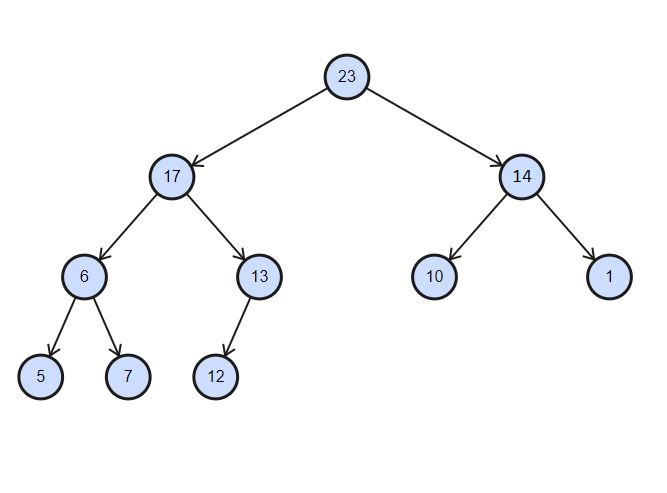
\includegraphics[width=0.9\textwidth]{heap.JPG}
\end{solutionorbox}

\ifprintanswers
\newpage
\else
\bigskip
\fi


%%%%%%%%%%%%%%%%%%%%%%%%%%%%%%%%%%%%%%%%%%%%%%%%%%%%%%%%%%%%%%%%%%
%
% Question 4
%
%%%%%%%%%%%%%%%%%%%%%%%%%%%%%%%%%%%%%%%%%%%%%%%%%%%%%%%%%%%%%%%%%%
\question[5]
6.2-1.  Using Figure 6.2 as a model, illustrate (with computer software) the operation of $\proc{Max-Heapify}{(A,3)}$ on the array $A = \left< 27, 17, 3, 16, 13, 10, 1, 5, 7, 12, 4, 8, 9, 0\right>$.

\begin{solutionorbox} \\
	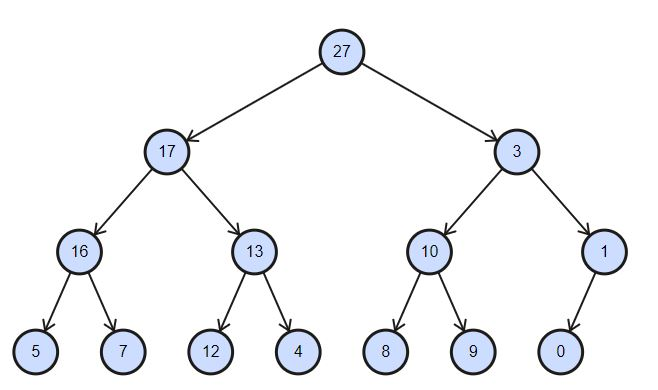
\includegraphics[width=0.5\textwidth]{step1.JPG}
	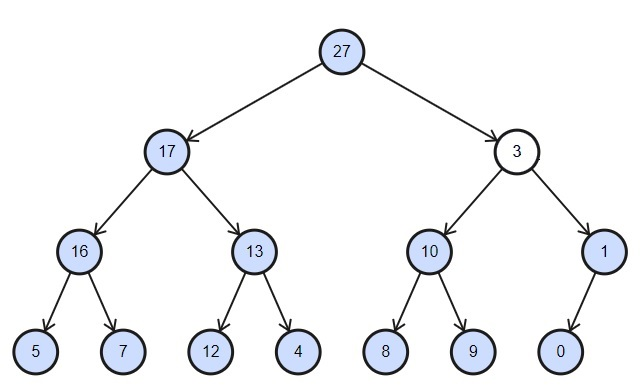
\includegraphics[width=0.5\textwidth]{step2.jpg}
	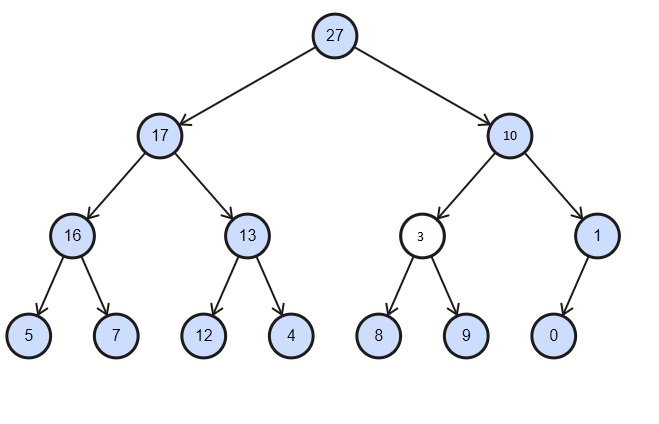
\includegraphics[width=0.5\textwidth]{step3.jpg}
	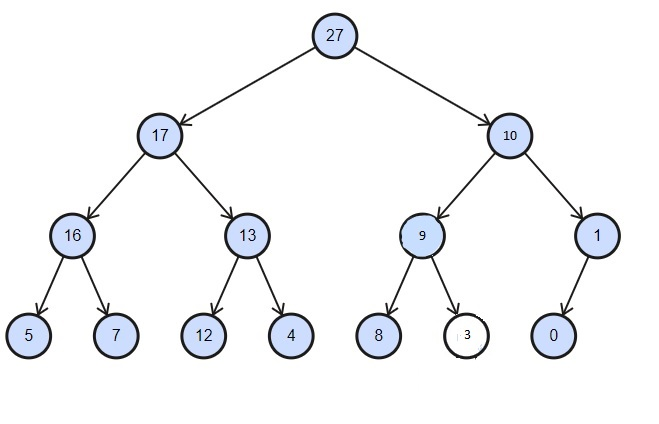
\includegraphics[width=0.5\textwidth]{step4.jpg}
\end{solutionorbox}

\ifprintanswers
\newpage
\else
\bigskip
\fi


%%%%%%%%%%%%%%%%%%%%%%%%%%%%%%%%%%%%%%%%%%%%%%%%%%%%%%%%%%%%%%%%%%
%
% Question 5
%
%%%%%%%%%%%%%%%%%%%%%%%%%%%%%%%%%%%%%%%%%%%%%%%%%%%%%%%%%%%%%%%%%%
\question[5]
6.2-2.  Starting with the procedure $\proc{Max-Heapify}{(A,i)}$, write pseudocode for the procedure $\proc{Min-Heapify}{(A,3)}$, which performs the corresponding manipulation on a min-heap.  How does the running time of $\proc{Min-Heapify}{(A,3)}$ compare to that of $\proc{Max-Heapify}{(A,3)}$?

\begin{solutionorbox}
	\begin{lstlisting}[mathescape=true]
	$\proc{Min-Heapify}{(A,i)}$
            l = $\proc{Left}{(i)}$
            r = $\proc{Right}{(i)}$
            if l $\leq$ A.heap-size and A[l] < A[i]
                smallest = l
            else
                smallest = i
            if r $\leq$ A.heap-size and A[r] < A[smallest]
                smallest = r
            if smallest $\neq$ i
                exchange A[i] with A[smallest]
                $\proc{Min-Heapify}{(A,smallest)}$
	\end{lstlisting} \\
	The running time of $\proc{Min-Heapify}{(A,i)}$ and $\proc{Max-Heapify}{(A,i)}$ are the same. The two algorithms are nearly identical except for the comparisons being changed to less than rather than greater than.
\end{solutionorbox}

\ifprintanswers
\newpage
\else
\bigskip
\fi


%%%%%%%%%%%%%%%%%%%%%%%%%%%%%%%%%%%%%%%%%%%%%%%%%%%%%%%%%%%%%%%%%%
%
% Question 6
%
%%%%%%%%%%%%%%%%%%%%%%%%%%%%%%%%%%%%%%%%%%%%%%%%%%%%%%%%%%%%%%%%%%
\question[5]
6.3-1.  Using Figure 6.3 as a model, illustrate (using computer software) the operation of $\proc{Build-Max-Heap}$ on the array $A = \left< 5, 3, 17, 10, 84, 19, 6, 22, 9\right>$

\begin{solutionorbox} \\ 
	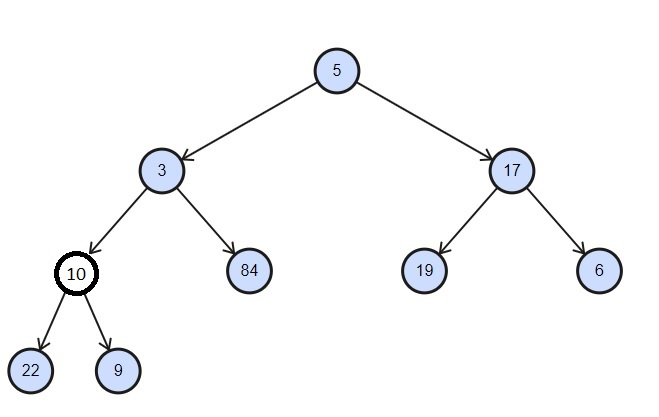
\includegraphics[width=0.5\textwidth]{bmh1.jpg}
	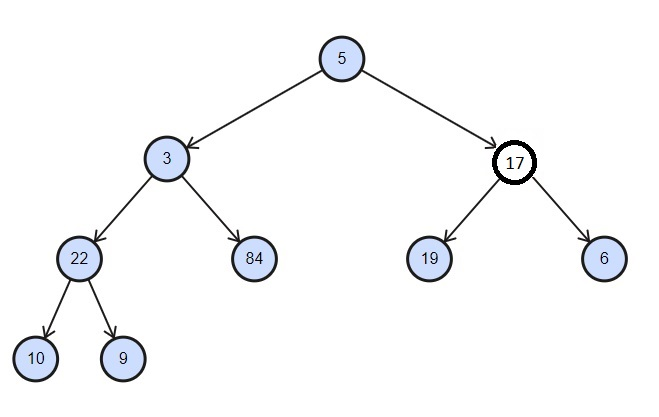
\includegraphics[width=0.5\textwidth]{bmh2.jpg}
	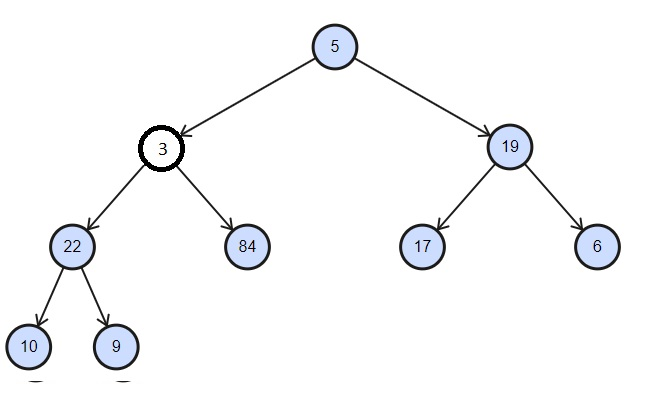
\includegraphics[width=0.5\textwidth]{bmh3.jpg}
	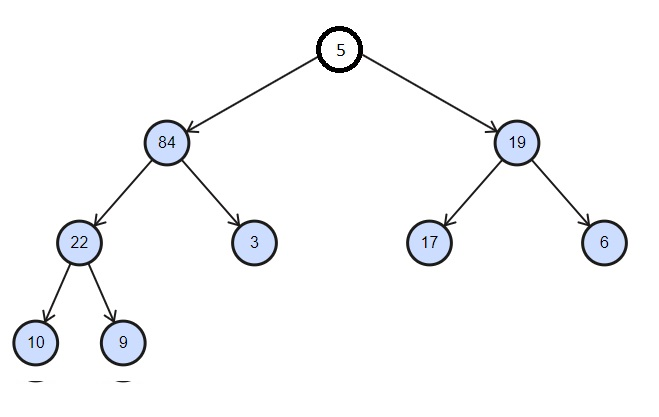
\includegraphics[width=0.5\textwidth]{bmh4.jpg}
	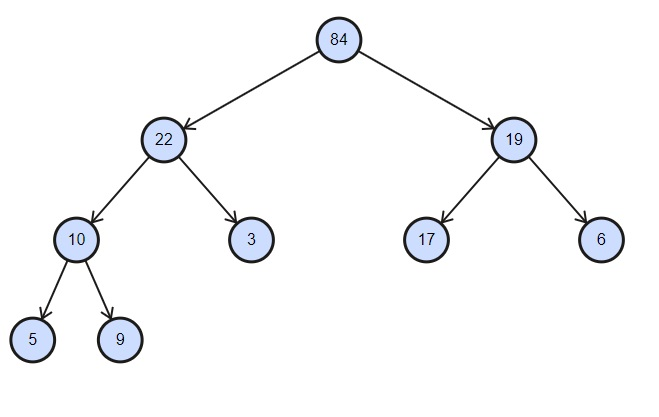
\includegraphics[width=0.5\textwidth]{bmh5.jpg}
\end{solutionorbox}

\ifprintanswers
\newpage
\else
\bigskip
\fi


%%%%%%%%%%%%%%%%%%%%%%%%%%%%%%%%%%%%%%%%%%%%%%%%%%%%%%%%%%%%%%%%%%
%
% Question 7
%
%%%%%%%%%%%%%%%%%%%%%%%%%%%%%%%%%%%%%%%%%%%%%%%%%%%%%%%%%%%%%%%%%%
\question[5]
6.3-2.  Why do we want the loop index $i$ in line 3 of $\proc{Build-Max-Heap}$ to decrease from $\floor{A.length/2}$ to 1 rather than increase from 1 to $\floor{A.length/2}$?

\begin{solutionorbox} \\
	The subarray of elements in an $n$-element heap $A = \left< (\floor{n/2} + 1) ... n \right>$ are all the leaves of the tree in which each form a 1-element heap to begin with. If we were to begin the loop from 1 and increase to $\floor{A.length/2}$, there is no certainty that the subtrees are max heaps. In order for $\proc{Build-Max-Heap}$ to work, we must be certain that the children of a node are heapified before the node and the requirement for $\proc{Max-Heapify}$ to work is fulfilled for each node. Explicitly, the loop invariant: \\
	At the start of each iteration of the for loop of lines 2-3, each node $i + 1, i + 2, ..., n$ is the root of a max-heap will only be met if we loop in reverse order.
\end{solutionorbox}

\ifprintanswers
\newpage
\else
\bigskip
\fi


%%%%%%%%%%%%%%%%%%%%%%%%%%%%%%%%%%%%%%%%%%%%%%%%%%%%%%%%%%%%%%%%%%
%
% Question 8
%
%%%%%%%%%%%%%%%%%%%%%%%%%%%%%%%%%%%%%%%%%%%%%%%%%%%%%%%%%%%%%%%%%%
\question[5]
6.4-1.  Using Figure 6.4 as a model, illustrate (with computer software) the operation of $\proc{Heapsort}$ on the array $A = \left< 5, 13, 2, 25, 7, 17, 20, 8, 4 \right>$.

\begin{solutionorbox}\\
	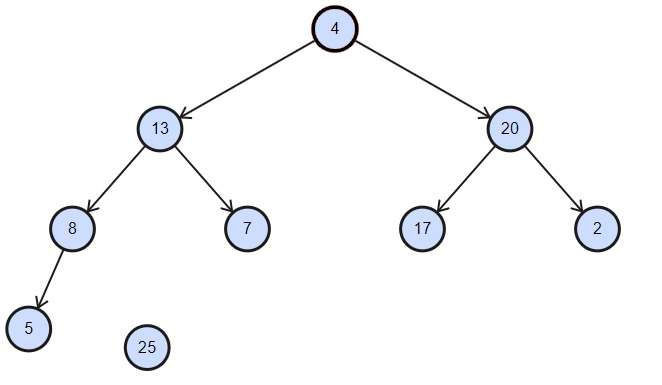
\includegraphics[width=0.5\textwidth]{heapsort1.jpg}
	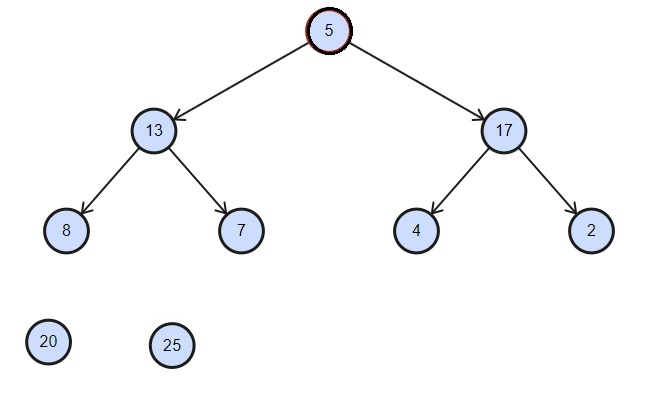
\includegraphics[width=0.5\textwidth]{heapsort2.jpg}
	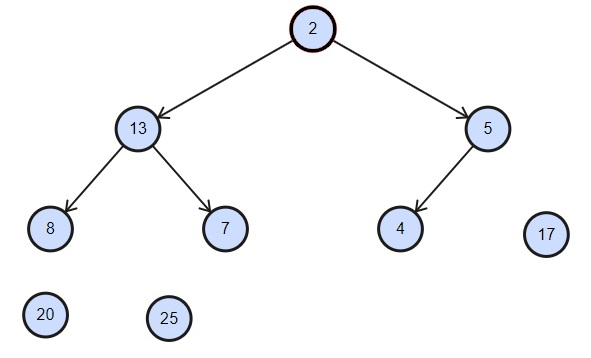
\includegraphics[width=0.5\textwidth]{heapsort3.jpg}
	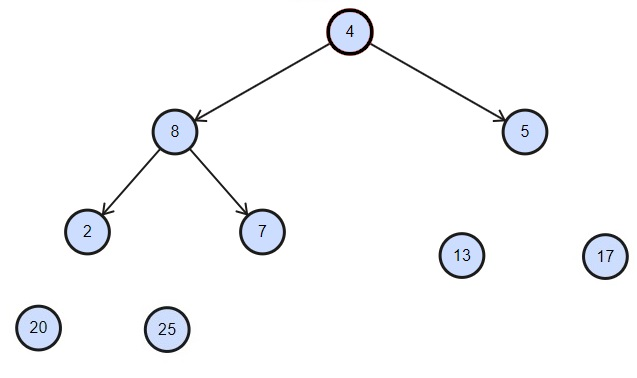
\includegraphics[width=0.5\textwidth]{heapsort4.jpg}
	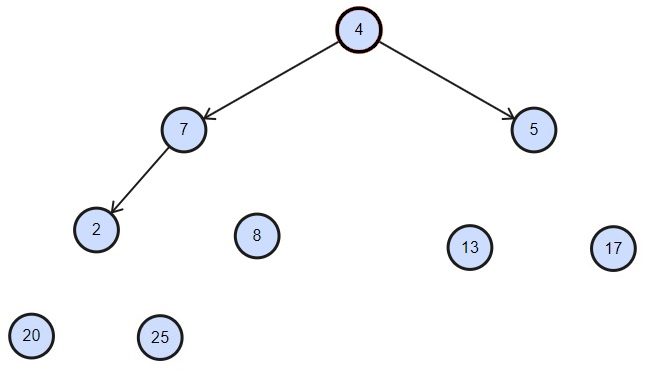
\includegraphics[width=0.5\textwidth]{heapsort5.jpg}
	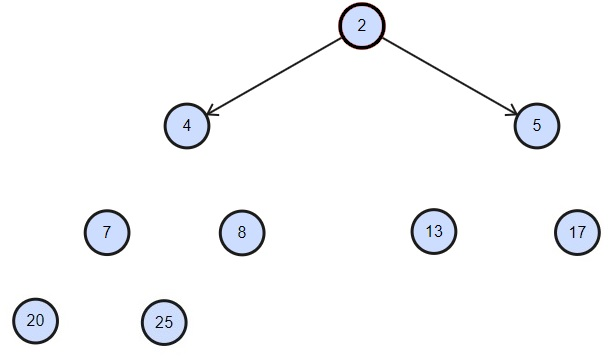
\includegraphics[width=0.5\textwidth]{heapsort6.jpg}
	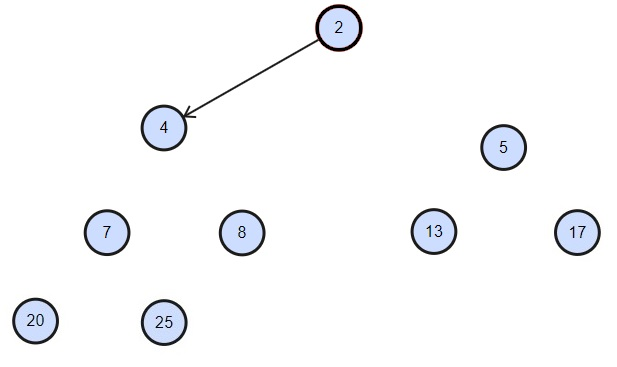
\includegraphics[width=0.5\textwidth]{heapsort7.jpg}
	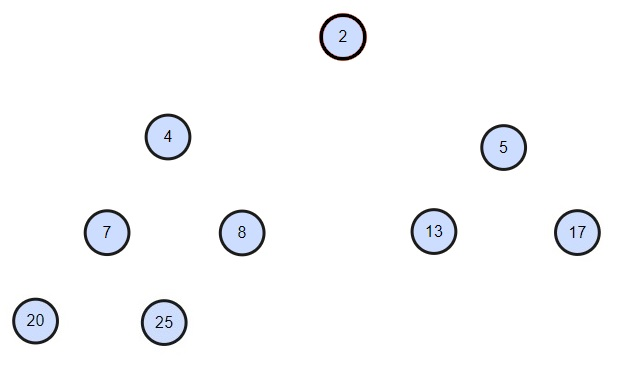
\includegraphics[width=0.5\textwidth]{heapsort8.jpg}
	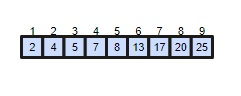
\includegraphics[width=0.5\textwidth]{heapsort9.jpg}
\end{solutionorbox}

\ifprintanswers
\newpage
\else
\bigskip
\fi


%%%%%%%%%%%%%%%%%%%%%%%%%%%%%%%%%%%%%%%%%%%%%%%%%%%%%%%%%%%%%%%%%%
%
% Question 9
%
%%%%%%%%%%%%%%%%%%%%%%%%%%%%%%%%%%%%%%%%%%%%%%%%%%%%%%%%%%%%%%%%%%
\question[5]
6.4-3.  What is the running time of $\proc{Heapsort}$ on an array $A$ of length $n$ that is already sorted in increasing order?  What about decreasing order?

\begin{solutionorbox}
	The running time of $\proc{Heapsort}$ on an array $A$ of length $n$ that is already sorted in increasing order is $\Theta(n \lg n)$ because even though it already sorted, it will be turned back into a heap and then sorted.\\ \\
	The running time of $\proc{Heapsort}$ on an array $A$ of length $n$ that is sorted in decreasing order will also be $\Theta(n \lg n)$. This occurs because even though the heap will be built in linear time, every time the $max$ element is removed and $\proc{Heapify}$ is called, it will cover the full height of the tree.
\end{solutionorbox}

\ifprintanswers
\newpage
\else
\bigskip
\fi





\end{questions}
\end{document}
